\begin{figure}[t]
\centering
\subfigure[]{\begin{minipage}[t][2.75cm]{0.2\textwidth}
  $\begin{aligned}
    \gls{Smaske} = \begin{bmatrix}
      1 & 1 & 2 & 3\\
      1 & 2 & 2 & 3\\
      1 & 1 & 4 & 4
    \end{bmatrix}
  \end{aligned}$
\end{minipage}
\begin{tikzpicture}[overlay]
  \draw[thick] (-1.60, 0.39)   -- (-1.1,  0.39);
  \draw[thick] (-1.60, -0.125) -- (-0.03, -0.125);
\end{tikzpicture}
}
\subfigure[]{\begin{minipage}[t][3.7cm]{0.35\textwidth}
  $\begin{aligned}
    \gls{Smaske}_{\uparrow} = & \begin{bmatrix}
        1 & 2 & 2 & 3\\
        1 & 1 & 4 & 4
      \end{bmatrix}\\
        \gls{Smaske}_{\downarrow} = & \begin{bmatrix}
        1 & 1 & 2 & 3\\
        1 & 2 & 2 & 3
      \end{bmatrix}\\
      \left(\gls{Smaske}_{\uparrow} \neq \gls{Smaske}_{\downarrow}\right) = & \begin{bmatrix}
        \times & \checkmark & \times & \times\\
        \times & \checkmark & \checkmark & \checkmark\\
      \end{bmatrix}
  \end{aligned}$
\end{minipage}
}
\subfigure[]{\begin{minipage}[t][3.6cm]{0.35\textwidth}
  $\begin{aligned}
    \left(2,1\right) \in \gls{E},\,\,\,\, & \left(1,2\right) \in \gls{E}\\
    \left(4,2\right) \in \gls{E},\,\,\,\, & \left(4,3\right) \in \gls{E}\\
    \left(\gls{A} \vee \gls{A}^{\top}\right) = & \begin{bmatrix}
      0 & 1 & 0 & 0\\
      1 & 0 & 0 & 1\\
      0 & 0 & 0 & 1\\
      0 & 1 & 1 & 0
    \end{bmatrix}
  \end{aligned}$
\end{minipage}
}
  \caption[Effiziente Adjazenzbestimmung einer Segmentierungsmaske]{Adjazenzbestimmung einer Segmentierungsmaske $\gls{Smaske} \in {\left\{1,2,3,4\right\}}^{3 \times 4}$ mit eingezeichneten vertikalen Adjazenzen (a).
  Daraus lassen sich $\gls{Smaske}_{\uparrow}$, $\gls{Smaske}_{\downarrow}$ sowie die boolsche Matrix $\left(\gls{Smaske}_{\uparrow} \neq \gls{Smaske}_{\downarrow}\right)$ bestimmen (b).
  Die Einträge in $\gls{Smaske}_{\uparrow}$ und $\gls{Smaske}_{\downarrow}$ an den Indizes der wahren Werte in $\gls{Smaske}_{\uparrow} \neq \gls{Smaske}_{\downarrow}$ bilden jeweils eine Kante im Graphen (c).}
\label{fig:adjazenz}
\end{figure}
